	\documentclass[10pt,conference]{IEEEtran}
\usepackage{float}
\usepackage{cite}
\usepackage{tikz}
\usepackage{pgfplots}
\usepackage{longtable}
\ifCLASSINFOpdf
   \usepackage[pdftex]{graphicx}
   \graphicspath{{figs/}}
   \DeclareGraphicsExtensions{.pdf,.jpeg,.png}
\else
   \usepackage[dvips]{graphicx}
   \graphicspath{{../figs/}}
   \DeclareGraphicsExtensions{.eps}
\fi

\usepackage[cmex10]{amsmath}
\interdisplaylinepenalty=2500
\usepackage{amsthm}
\newtheorem{definition}{Definition}
\usepackage{algorithmic}
\usepackage{array}
\usepackage{subcaption}
\usepackage{url}
\usepackage[T1]{fontenc}
\usepackage[utf8]{inputenc}
\usepackage[brazilian]{babel}
\usepackage{listings}
\lstset{
  language=C++,
  basicstyle=\ttfamily\footnotesize,
  keywordstyle=\color{blue}\bfseries,
  commentstyle=\color{green!40!black},
  stringstyle=\color{orange},
  showstringspaces=false,
  breaklines=true,
  frame=single,
  literate=%
    {á}{{\'a}}1
    {à}{{\`a}}1
    {ã}{{\~a}}1
    {é}{{\'e}}1
    {ê}{{\^e}}1
    {í}{{\'i}}1
    {ó}{{\'o}}1
    {õ}{{\~o}}1
    {ú}{{\'u}}1
    {ü}{{\"u}}1
    {ç}{{\c{c}}}1
}
\usepackage{xcolor}
\lstset { %
    language=C++,
    backgroundcolor=\color{black!5}, % set backgroundcolor
    basicstyle=\footnotesize,% basic font setting
}
\usepackage{minted}
\usepackage[most]{tcolorbox}
\definecolor{lightgreen}{rgb}{0.56, 0.93, 0.56}
\definecolor{moonstoneblue}{rgb}{0.45, 0.66, 0.76}


% corrija hifenação aqui
\hyphenation{op-tical net-works semi-conduc-tor}

\begin{document}
\title{Relatório - Trabalho Prático I}

\newif\iffinal
\finalfalse
\finaltrue
\newcommand{\jemsid}{99999}

\iffinal
\author{\IEEEauthorblockN{Henrique Oliveira da Cunha Franco}
\IEEEauthorblockA{Ciência da Computação \\
Pontifícia Universidade Católica de Minas Gerais\\
1448652@sga.pucminas.br}
\and
\IEEEauthorblockN{Bernardo Augusto Amorim Vieira}
\IEEEauthorblockA{Ciência da Computação\\
Pontifícia Universidade Católica de Minas Gerais\\
1449516@sga.pucminas.br}
}


\else
  \author{Sibgrapi paper ID: \jemsid \\ }
\fi


\maketitle

\begin{abstract}
O estudo de grafos biconexos, também conhecidos como 2-conexos, tem relevância em várias áreas da Computação, pois tais grafos são tolerantes a falhas, permitindo a existência de múltiplos caminhos entre vértices. O objetivo deste trabalho é desenvolver e comparar três métodos de identificação de componentes biconexos em grafos, os quais têm aplicações práticas como em redes de comunicação. O primeiro método verifica a existência de dois caminhos internamente disjuntos entre pares de vértices. O segundo identifica articulações, testando a conectividade do grafo após a remoção de vértices. O terceiro implementa o algoritmo eficiente de Tarjan (1972)\cite{4569669}, amplamente reconhecido na literatura. A avaliação dos três métodos será realizada por meio de experimentos que medem o tempo de execução médio em grafos aleatórios de 10 a 100.000 vértices. Os resultados esperados incluem uma análise comparativa do desempenho e da escalabilidade dos algoritmos.
\end{abstract}
\IEEEpeerreviewmaketitle

\section{Introdução}

A motivação deste trabalho reside na importância dos grafos biconexos em diversas áreas da Computação, especialmente em sistemas que exigem tolerância a falhas. Um grafo biconexo mantém conectividade mesmo após a remoção de qualquer vértice, sendo útil em redes de comunicação e sistemas distribuídos. O problema estudado é a identificação eficiente de componentes biconexos em grafos. A dificuldade principal está em encontrar um método eficiente para grafos de grande porte, dado o custo computacional envolvido nas verificações necessárias. A solução proposta envolve a implementação de três métodos distintos: verificação de caminhos internamente disjuntos, teste de articulações e o algoritmo de Tarjan (1972). A eficácia desses métodos será avaliada por meio de experimentos que medirão o tempo médio de execução em grafos de tamanhos variados, permitindo comparar o desempenho de cada abordagem.

\section{Métodos}

Para testar a eficácia individualmente de cada um dos métodos propostos na tarefa, realizaremos os seguintes experimentos:

\begin{enumerate}
\item Verificar a identificação correta de componentes biconexos em grafos aleatórios com diferentes tamanhos (10,50,100,500, 1.000, 10.000, 100.000 vértices).
\item Avaliar o tempo de execução médio de cada um dos métodos.
%\item Testar a robustez dos métodos em situações que envolvam grafos com poucas arestas ou grafos densos.
\end{enumerate}

\newpage

Antes de introduzir os métodos individualmente e apresentar suas implementações, é de crucial importância apresentar a estrutura básica inicial que foi usada nos métodos. Os códigos foram feitos na linguagem C\texttt{++}, e usamos os seguintes pacotes:

\begin{minted}{cpp}
#include <iostream>
#include <vector>
#include <random>
#include <set>
#include <ctime>
#include <stack>
#include <chrono>
#include <queue>
#include <unordered_set>
#include <unordered_map>
#include <algorithm>
\end{minted}

A estrutura fundamental é implementada da seguinte maneira:

\begin{lstlisting}
using namespace std;

class Graph
{
public:
    int vertices;
    vector<set<int>> adjList;
    // Usando set para evitar arestas duplicadas

    Graph(int vertices) : vertices(vertices)
    {
        adjList.resize(vertices);
        TT.resize(vertices);
        TD.resize(vertices);
        pai.resize(vertices - 1);
        LOWPT.resize(vertices);
    }
}
\end{lstlisting}

Ainda dentro da classe, existem diversos métodos que auxiliam na manipulação do grafo, bem como seus vértices e arestas. Alguns deles são:

\begin{lstlisting}[caption={Método para adicionar arestas},captionpos=b]
    void addEdge(int u, int v)
    {
        if (u >= vertices || v >= vertices)
            return;        
        adjList[u].insert(v);
        adjList[v].insert(u);
        // Para um grafo não direcionado
    }
\end{lstlisting}

\newpage

\begin{lstlisting}[caption={Método que retorna a vizinhança de um dado vértice},captionpos=b]
    const set<int> &getVizinhos(int v) const
    {
        return adjList[v];
    }
\end{lstlisting}

\begin{lstlisting}[caption={Retorna número de vértices (N) do grafo},captionpos=b]
    int getNumVertices() const
    {
        return vertices;
    }
    \end{lstlisting}

\begin{lstlisting}[caption={Retorna vetor de vértices do grafo},captionpos=b]
set<int> getVertices()
    {
        set<int> Vertices;
        for (int i = 0; i < vertices; ++i)
        {

            if (!adjList[i].empty())
            {
                Vertices.insert(i);
            }
        }
        return Vertices;
    }
\end{lstlisting}

Além do que já foi introduzido, são inicializados alguns atributos relacionados às buscas e, adicionalmente, o vetor LOWPT, que é usado na busca do método de Tarjan.

\begin{lstlisting}
    int t = 0;
    vector<int> TD;
    vector<int> TT;
    vector<int> pai;
    vector<int> LOWPT;
    stack<pair<int, int>> edges;

    vector<int> getSucessores(int vertice) const
    {
        vector<int> sucessores;
        for (int neighbor : adjList[vertice])
        {
            sucessores.push_back(neighbor);
        }
        return sucessores;
    }

    void printSucessores(int vertice) const
    {
        cout << "Sucessores de " << vertice << ": ";
        for (int neighbor : adjList[vertice])
        {
            cout << neighbor << " ";
        }
        cout << endl;
    }
\end{lstlisting}

\newpage
Adicionalmente, temos a classe auxiliar Edge (aresta).

\begin{lstlisting}
class Edge
{
public:
    int u, v;
    Edge(int u, int v) : u(min(u, v)),
                         v(max(u, v)) {} 
    // Ordena u e v

    // O método abaixo é necessário para que o set
    // de arestas funcione corretamente, e o que ele
    // faz é comparar as arestas
    bool operator==(const Edge &other) const
    {
        return u == other.u && v == other.v;
    }

    // O método abaixo é necessário para que o set
    // de arestas funcione corretamente e, o que ele
    // faz é ordenar as arestas
    bool operator<(const Edge &other) const
    {
        return tie(u, v) < tie(other.u, other.v); 
        // Comparação ordenada
    }
};
\end{lstlisting}

Por fim, temos a classe Conjuntos, para lidar (especificamente, no método 1) com estruturas complexas como componentes.

\begin{lstlisting}
class Conjuntos
{
public:
    vector<set<Edge>> componentes;
    // Usar set para evitar duplicação de arestas

    Conjuntos(int n)
    {
        componentes.resize(n);
    }

    void add(int component, const Edge &edge)
    {
        if (component < componentes.size())
        {
            componentes[component].insert(edge);
            // Arestas duplicadas serão
            // ignoradas automaticamente
        }
    }
};
\end{lstlisting}

\newpage

\subsection{Método 1: Verificação de dois caminhos internamente disjuntos}
Vale notar, primeiramente, que para cada método, há uma classe separada, a fim de deixar o código organizado e bem modularizado, de maneira que seja fácil testar a execução de cada algoritmo para os mesmos grafos. Começando pelo método 1, este método verifica se, para cada par de vértices em um grafo, existem dois caminhos que não compartilham vértices internos. Isso garante que os vértices fazem parte de uma mesma componente biconexo.

\textbf{Explicação:} A classe começa declarando um vetor de conjuntos de arestas, `componentes`, onde cada posição do vetor armazena um conjunto de arestas pertencente a um bloco. O método `add` adiciona uma nova aresta ao componente indicado, e o `set` evita a duplicação de arestas.

\subsubsection{Método specialDFS}

O método `specialDFS` implementa uma busca em profundidade (DFS) modificada, que verifica se existe um caminho entre dois vértices (`initial` e `target`) ignorando um vértice intermediário (`avoiding`).

\begin{lstlisting}
bool specialDFS(int initial, int target, int avoiding) {
    stack<int> stack;
    stack.push(initial);

    while (!stack.empty()) {
        int current = stack.top();
        stack.pop();

        if (current == target) {
            return true;
        }

        if (!visited[current]) {
            visited[current] = true;

            for (int neighbor : lista.getVizinhos(current)) {
                if (neighbor == avoiding)
                    continue;
                if (current == initial && neighbor == target)
                    continue;
                if (!visited[neighbor]) {
                    stack.push(neighbor);
                }
            }
        }
    }
    return false;
}
\end{lstlisting}

\textbf{Explicação:} Este método usa uma pilha para simular a recursão da DFS. Ele procura por um caminho do vértice `initial` ao `target`, ignorando o vértice `avoiding`. O uso de uma pilha e uma lista de vértices visitados (`visited`) permite uma execução iterativa.

\newpage

\subsubsection{Método isNeighbourhoodInCycle}

Este método verifica se dois vértices são parte de um ciclo, ou seja, se há um caminho que conecta esses dois vértices sem que um vértice seja repetido.

\begin{lstlisting}
bool isNeighbourhoodInCycle(int v, int w) {
    visited.assign(lista.getNumVertices(), false); // Garante o tamanho correto de 'visited'
    return specialDFS(v, w, -1);
}
\end{lstlisting}

\textbf{Explicação:} A função reinicializa o vetor `visited` e invoca o `specialDFS`, passando -1 como vértice a evitar, o que indica que não há restrições de vértices a ignorar. Isso verifica se os dois vértices estão conectados em um ciclo.

\subsubsection{Método isParentAndSonInCycle}

\begin{lstlisting}
bool isParentAndSonInCycle(int v, int w, int son) {
    visited.assign(lista.getNumVertices(), false); // Garante o tamanho correto de 'visited'
    return specialDFS(v, w, son);
}
\end{lstlisting}


\textbf{Explicação:}
O método `isParentAndSonInCycle` verifica se dois vértices, `v` e `w`, estão em um ciclo, ignorando uma aresta específica que conecta um vértice pai (`v`) e um filho (`son`). Essa função é usada quando é importante saber se, ao remover a conexão entre um vértice e seu filho, os dois vértices ainda fazem parte de um ciclo.

- A função primeiro reinicializa o vetor `visited`, que rastreia quais vértices já foram visitados durante a busca. O `visited` é ajustado para ter o tamanho correto de acordo com o número de vértices do grafo (`lista.getNumVertices()`).
  
- Em seguida, ela chama a função `specialDFS(v, w, son)`, que realiza uma busca em profundidade (DFS) modificada para verificar se existe um caminho entre os vértices `v` e `w`, mas ignorando a aresta que liga o vértice `v` ao seu filho `son`.

Se a função `specialDFS` retornar `true`, significa que `v` e `w` ainda estão conectados, mesmo sem a aresta entre `v` e `son`, indicando que eles estão em um ciclo. Se retornar `false`, significa que não há ciclo.

\subsubsection{Método addVertice}

O método `addVertice` é responsável por adicionar vértices a um ciclo específico, garantindo que todos os vértices do ciclo sejam adicionados corretamente ao conjunto `currentCycleVertices`.

\begin{lstlisting}
void addVertice(int start, unordered_set<int> &currentCycleVertices) {
    stack<int> stack;
    stack.push(start);

    while (!stack.empty()) {
        int v = stack.top();
        stack.pop();

        if (!currentCycleVertices.count(v)) {
            currentCycleVertices.insert(v);
            addedVertices.insert(v);

            for (int neighbor : lista.getVizinhos(v)) {
                if (currentCycleVertices.count(neighbor))
                    continue;
                if (currentCycleVertices.size() < 2) {
                    if (isNeighbourhoodInCycle(v, neighbor)) {
                        stack.push(neighbor);
                    }
                } else {
                    if (isParentAndSonInCycle(start, neighbor, v)) {
                        stack.push(neighbor);
                    }
                }
            }
        }
    }
}
\end{lstlisting}

\textbf{Explicação:} Este método faz uma busca a partir do vértice `start` para encontrar e adicionar todos os vértices que fazem parte de um ciclo, armazenando-os no conjunto `currentCycleVertices`. Ele utiliza uma pilha e as funções auxiliares `isNeighbourhoodInCycle` e `isParentAndSonInCycle` para verificar se os vértices pertencem ao ciclo.

\subsubsection{Método execute}

O método `execute` é o ponto principal da classe. Ele percorre todos os vértices do grafo, usando a função `addVertice` para encontrar e adicionar os vértices de um ciclo e suas arestas correspondentes ao componente correto.

\begin{lstlisting}
void execute() {
    Conjuntos conjuntos(lista.getNumVertices());
    unordered_set<int> currentCycleVertices;

    for (int i = 0; i < lista.getNumVertices(); i++) {
        for (int neighbor : lista.getVizinhos(i)) {
            if (i != neighbor) {
                edges.insert(Edge(i, neighbor));
            }
        }
    }

    int currentComponent = -1;

    for (int i = 0; i < lista.getNumVertices(); i++) {
        if (!addedVertices.count(i)) {
            currentCycleVertices.clear();
            visited.assign(lista.getNumVertices(), false);

            addVertice(i, currentCycleVertices);

            currentComponent++;
            for (int vertex : currentCycleVertices) {
                for (int neighbor : lista.getVizinhos(vertex)) {
                    if (currentCycleVertices.count(neighbor)) {
                        conjuntos.add(currentComponent, Edge(vertex, neighbor));
                        edges.erase(Edge(vertex, neighbor));
                    }
                }
            }
        }
    }

    for (const Edge &edge : edges) {
        currentComponent++;
        conjuntos.add(currentComponent, edge);
    }
}
\end{lstlisting}

\textbf{Explicação:} O método `execute` percorre todos os vértices do grafo, verificando se já foram adicionados ao conjunto de vértices processados. Se não, ele invoca `addVertice` para encontrar o ciclo em que o vértice está envolvido. No final, todas as arestas que não formam ciclos são adicionadas a novos componentes.
o

\subsection{Método 2: Identificação de articulações}
Este método testa a conectividade do grafo após a remoção de cada vértice, identificando vértices cuja remoção aumentaria o número de componentes conexos, caracterizando-os como articulações.

A ideia por trás do código é a seguinte, é recebido um grafo como argumento na função, e esse grafo é empilhado, entrando em um loop enquanto a pilha não estiver vazia, como diz o algoritmo: \begin{lstlisting}
    
    void getComponentByCut(Graph g, 
    vector<vector<set<int>>> &Blocos)
{
    stack<Graph> pilhaDeGrafos;
    pilhaDeGrafos.push(g); 
    vector<int> vertices;  

  
    while (!pilhaDeGrafos.empty())
    {
        Graph gLinha = pilhaDeGrafos.top();
        pilhaDeGrafos.pop();                

        bool encontrouArticulacao = false;
            //.
            //.
            //.
            //.
\end{lstlisting}

É feito uma verificação em cada vértice do grafo, para saber se o mesmo é uma articulação,se o vértice for uma articulação,
é passado como parâmetro também uma lista de vértices, indicando um possível componente biconexo. \begin{lstlisting}
    for (int v : gLinha.getVertices())
    {
    if (gLinha.isArticulation(v, vertices))
            {   //.
                //.
                //.
                //.
\end{lstlisting}

A função funciona da seguinte forma, o vértice é cortado do grafo juntamente com suas arestas: \begin{lstlisting}
    set<int> originalAdjList = adjList[vertice];
        for (int neighbor : originalAdjList)
        {
            adjList[neighbor].erase(vertice);
        }
        adjList[vertice].clear();
\end{lstlisting}
Uma busca em profundidade é realizada nesse grafo, e se o número de vértices encontrados for menor do que o número de vértices - 1, o vértice é uma articulação:
\begin{lstlisting}
     int Count = 0;

        ChamadaInicial(Count, subgraph);

\end{lstlisting}

Após isso o vértice é recolocado no grafo e um valor "booleano" é retornado:
\begin{lstlisting}
    adjList[vertice] = originalAdjList;
        for (int neighbor : originalAdjList)
        {
            adjList[neighbor].insert(vertice);
        }
        set<int> size = getVertices();
        return Count + 1 < size.size() - 1; // 1 a 
       // mais por conta do metodo 
       // nao contar o nó raiz
\end{lstlisting}

Após isso, o grafo é separado em 2 subgrafos, um contendo os vértices encontrados na DFS, e outro contendo todos menos esses, com a articulação presente em todos:

\begin{lstlisting}//.
                //.
                //.
                //.
    auto [subgrafo1, subgrafo2] = 
    gLinha.separarGrafo(vertices, v);
\end{lstlisting}
A função funciona da seguinte forma, é feita uma primeira verificação para saber se a articulação é a única que une o grafo inteiro, como no exemplo:
\begin{figure}
    \centering
    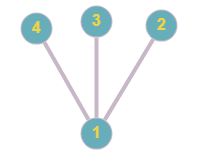
\includegraphics[width=0.5\linewidth]{figs/exampleGraph.png}
    \caption{Articulação ligando todos os vértices}
    \label{fig::graphArt}
\end{figure}
Isso deve ser feito, pois se não a DFS não encontraria ninguém. A lógica funciona da seguinte forma, se grau do vértice for n - 1 (sendo n o número de vértices), ele captura as arestas da articulação e a cada iteração ele balanceia as arestas, uma para cada subgrafo, como no exemplo a seguir:
\begin{figure}
    \centering
    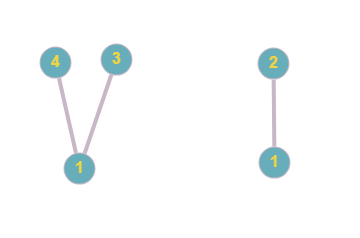
\includegraphics[width=0.5\linewidth]{figs/subgraphExample.png}
    \caption{Subgrafos gerados a partir do grafo da figura \ref{fig::graphArt}}
    \label{fig:enter-label}
\end{figure}
O algoritmo se encontra a seguir:

\newpage

\begin{lstlisting}
    // Inicializa os subgrafos com o mesmo
    //número de vértices que o grafo original
    
    Graph subgraph1(vertices);
    Graph subgraph2(vertices);
    
    // Verifica se há exatamente 3 vértices
    //e se o vértice comum tem grau 2
    
    if (adjList[verticeComum].size() == 
    getVertices().size() - 1) {
    
        set<int> sucessor1 = 
        adjList[verticeComum];
        int cont = 0;
        
        for(std::set<int>::iterator it = 
        sucessor1.begin(); 
        it != sucessor1.end(); it++){
            if(cont % 2 == 0){
             subgraph1.addEdge(verticeComum, 
             *it);
            }
            else{
            subgraph2.addEdge(verticeComum, 
            *it);
            }
            cont++;
        }
            
            return {subgraph1,subgraph2};        
    }
\end{lstlisting}
O restante da função não será demonstrado por praticidade, o código fonte está com os devidos comentários.

Após isso, é realizado uma verificação se algum ou todos os subgrafos são componentes, para isso foi criada uma função "isComponente".

A função funciona assim, primeiramente é realizada uma verificação se o grafo for vazio, se ele for, falso é retornado. 
\begin{lstlisting}
    // Verifica se o subgrafo é vazio
    bool isEmpty = true;
    for (int i = 0; i < g.vertices; i++) {
        if (!g.adjList[i].empty()) {
            isEmpty = false;
            break;
        }
    }
    // Se o subgrafo for vazio, retorna false
    if (isEmpty) {
        return false;
    }
\end{lstlisting}

Após isso, a função verifica se existe dois caminhos disjuntos para cada par de vértice do bloco, com isso determinando se o subgrafo é um componente biconexo ou não.


\begin{lstlisting}
 for (int i = 0; i < g.vertices; i++) {
 for (int j = i + 1; j < g.vertices; j++) {
    // Verifica se ambos os vértices 
    //têm vizinhos (não são vazios)
        if (!g.adjList[i].empty() && 
         !g.adjList[j].empty()) {
    // Deve haver dois caminhos disjuntos
  if (!g.isThereTwoDisjointPaths(i, j, g)){
                return false; // Se não houver 
                }
            }
        }
    }
    return true;
\end{lstlisting}

A função "isThereTwoDisjointPaths"  funciona assim, é feita uma busca em largura, buscando um caminho de v para w, encontrando o caminho, o caminho é marcado e é realizada uma outra BFS, não passando pelo mesmo caminho. Se a segunda busca encontrar w, verdadeiro é retornado.

Voltando para a função principal, se o subgrafo é um componente, ele é inserido em um vetor de matrizes adjacentes, e o outro subgrafo é empilhado para passar pelo mesmo processo outra vez, e assim os componentes são listados, como no exemplo:
\begin{lstlisting}
    
    else if (isComponent(subgrafo1))
         { 
             Blocos.push_back(subgrafo1.adjList);
             pilhaDeGrafos.push(subgrafo2); 
                }
\end{lstlisting}
Se nenhum subgrafo é um componente, os dois são reempilhados, se os dois forem, os dois são adicionados ao vetor, e se nenhuma articulação é encontrada, o grafo é inserido no vetor.

\subsection{Método 3: Algoritmo de Tarjan (1972)}
O algoritmo de Tarjan utiliza uma busca em profundidade (DFS) para identificar componentes biconexos de forma eficiente, explorando a estrutura dos vértices de retorno e o conceito de low-point.

O algoritmo de Tarjan\cite{4569669} foi implementado com dita o artigo, a implementação segue as regras e as condições apresentadas por Tarjan.

\subsubsection{Classe M3}

A classe `M3` utiliza o algoritmo de Tarjan para encontrar componentes biconexos em um grafo. Ela mantém uma referência ao grafo (`lista`) e uma estrutura que armazena os componentes encontrados (`Components`).

\begin{lstlisting}
class M3 {
private:
    Graph &lista;
    vector<vector<pair<int, int>>> Components;
\end{lstlisting}

\textbf{Explicação:} A classe é inicializada com uma referência para o grafo e uma variável `Components`, que é um vetor de vetores. Cada componente é armazenado como um vetor de pares de inteiros, representando as arestas entre os vértices.

\subsubsection{Método Tarjan}

O método `Tarjan` implementa a lógica do algoritmo de Tarjan, que realiza uma busca em profundidade para identificar os componentes biconexos. Ele usa a técnica de manter os tempos de descoberta (`TD`) e os valores de `LOWPT`, que são utilizados para encontrar articulações e componentes.

\begin{lstlisting}
void Tarjan(Graph &g, int v, int u, vector<vector<pair<int, int>>> &Components) {
    g.t += 1;
    g.TD[v] = g.t;
    g.LOWPT[v] = g.TD[v];
    for (int w : g.getSucessores(v)) {
        if (g.TD[w] == 0) {
            g.edges.push(make_pair(v, w));
            Tarjan(g, w, v, Components);
            g.LOWPT[v] = min(g.LOWPT[v], g.LOWPT[w]);
            if (g.LOWPT[w] >= g.TD[v]) {
                vector<pair<int, int>> Component;
                pair<int, int> edge;
                int u1, u2;

                do {
                    edge = g.edges.top();
                    g.edges.pop();
                    Component.push_back(edge);
                    u1 = edge.first;
                    u2 = edge.second;
                } while (!g.edges.empty() && g.TD[u1] >= g.TD[w]);

                Components.push_back(Component);
            }
        } else if (w != u && g.TD[w] < g.TD[v]) {
            g.edges.push(make_pair(v, w));
            g.LOWPT[v] = min(g.LOWPT[v], g.TD[w]);
        }
    }
}
\end{lstlisting}

\textbf{Explicação:} Este é o coração do algoritmo de Tarjan. Ele funciona da seguinte forma:
- Incrementa o tempo de descoberta de cada vértice (`g.t`), atribui o valor a `TD[v]` e inicializa `LOWPT[v]` com o mesmo valor.
- Para cada vértice sucessor `w` de `v`, se `w` ainda não foi descoberto (`TD[w] == 0`), realiza uma chamada recursiva de `Tarjan`.
- Após a chamada recursiva, ajusta `LOWPT[v]` com o valor mínimo entre `LOWPT[v]` e `LOWPT[w]`.
- Se for encontrado um ponto de articulação, ou seja, `LOWPT[w] >= TD[v]`, as arestas do componente biconexo são retiradas da pilha `g.edges` e adicionadas ao vetor `Component`, que é posteriormente armazenado em `Components`.

\subsubsection{Método TarjanInicial}

O método `TarjanInicial` é responsável por iniciar o algoritmo de Tarjan para todos os vértices do grafo que ainda não foram descobertos (aqueles cujo `TD` é igual a 0).

\begin{lstlisting}
void TarjanInicial(Graph &g, int v, int u, vector<vector<pair<int, int>>> &Components) {
    for (int i = 0; i < g.TD.size(); i++) {
        if (g.TD[i] == 0) {
            g.t = 0;
            while (!g.edges.empty()) {
                g.edges.pop();
            }
            Tarjan(g, v, -1, Components);
        }
    }
}
\end{lstlisting}

\textbf{Explicação:} Este método percorre todos os vértices do grafo e chama o método `Tarjan` para os vértices que ainda não foram visitados (`g.TD[i] == 0`). Ele também reinicializa o contador de tempo `g.t` e esvazia a pilha de arestas antes de iniciar a busca.

\subsubsection{Método printComponents}

Este método imprime os componentes biconexos encontrados pelo algoritmo de Tarjan. Cada componente é uma lista de arestas, e o método percorre todos os componentes, imprimindo suas arestas.

\begin{lstlisting}
void printComponents(const vector<vector<pair<int, int>>> &Components) {
    for (int i = 0; i < Components.size(); ++i) {
        cout << "Componente " << i + 1 << ": ";
        for (const auto &edge : Components[i]) {
            cout << "(" << edge.first << ", " << edge.second << ") ";
        }
        cout << endl;
    }
}
\end{lstlisting}

\textbf{Explicação:} Este método percorre o vetor `Components` e imprime as arestas de cada componente biconexo. Para cada componente, ele imprime um número sequencial (começando de 1) e, em seguida, as arestas no formato `(v, w)`.

\subsubsection{Método execute}

O método `execute` inicia a execução do algoritmo de Tarjan, chamando `TarjanInicial`. Este método também poderia ser responsável por imprimir os componentes.

\begin{lstlisting}
void execute() {
    TarjanInicial(lista, 1, -1, Components);
    // printComponents(Components);
}
\end{lstlisting}

\textbf{Explicação:} Este método chama `TarjanInicial`, que por sua vez executa o algoritmo de Tarjan para identificar os componentes biconexos no grafo `lista`. O método de impressão dos componentes foi comentado, mas pode ser chamado diretamente após a execução, se necessário.

\section{Resultados}

Os resultados não foram tão bem quanto o esperado, o algoritmo de Tarjan e a Implementação 1 tiveram os resultados mais satisfatórios, enquanto a Implementação 2 teve um alto custo computacional, não sendo capaz de solucionar o problema em 10.000 e 100.000 vértices em tempo hábil.

\begin{longtable}{|c|c|c|c|}
    \hline
    Número de Vértices & Método 1 (ms) & Método 2 (ms) & Método 3 (ms) \\ \hline10 & 0.01692 & 0.05214 & 0.00216 \\ \hline
          50 & 0.24822 & 1.1673 & 0.01272 \\ \hline
          100 & 0.64668 & 12.6241 & 0.01812 \\ \hline
          500 & 14.54214 & 1214.99 & 0.08832 \\ \hline
          1000 & 52.918 & 8740.74 & 0.1749 \\ \hline
          10000 & 6119.16 & --- & 13.9128 \\ \hline
          100000 & --- & --- & 215.46 \\ \hline
    
\caption{Tempos de execução médio para 5 grafos aplicados nos 3 métodos}
\end{longtable}

\newpage

\section{Conclusão}
A análise realizada revela que o problema de determinar os blocos biconexos em um grafo pode ser abordado por diferentes métodos, cada um com suas particularidades em termos de complexidade e tempo de execução. Para grafos de grande escala, soluções que podem ser viáveis em instâncias menores tornam-se inviáveis devido ao alto custo computacional, evidenciando a necessidade de algoritmos mais eficientes. Entre os métodos avaliados, o algoritmo desenvolvido por Robert Tarjan, em 1972, demonstrou ser o mais eficaz. Sua abordagem, baseada em busca em profundidade e cálculo de low-points, oferece uma solução otimizada, com complexidade linear em relação ao número de vértices e arestas. Isso o torna particularmente adequado para grafos de grandes dimensões, onde o desempenho eficiente é essencial para garantir a escalabilidade. Assim, o algoritmo de Tarjan destaca-se como a melhor opção, consolidando-se como a escolha ideal para a análise de componentes biconexos em cenários onde a performance é um fator crítico.

\newpage

\begin{figure}[]
    \centering
    \begin{tikzpicture}
        \begin{axis}[
            width=0.8\textwidth,
            height=0.6\textwidth,
            xlabel={Número de vértices},
            ylabel={Tempo de execução (ms)},
            xmode=log,
            ymode=log,
            log basis x={10},
            log basis y={10},
            xtick={10,50,100,500,1000,10000,100000},
            xticklabels={10, 50, 100, 500, 1.000, 10.000, 100.000},
            legend style={at={(0.95,0.05)},anchor=south east},
            grid=both
        ]
        % Método 1: Verificação de Caminhos Disjuntos
        \addplot[
            color=blue,
            mark=square*,
            thick
        ] coordinates {
            (10, 0.01692)
            (50, 0.24822)
            (100, 0.64668)
            (500, 14.54214)
            (1000, 52.918)
            (10000, 6119.16)
        };
        \addlegendentry{Caminhos Disjuntos}

        % Método 2: Identificação de Articulações
        \addplot[
            color=red,
            mark=triangle*,
            thick
        ] coordinates {
            (10, 0.05214)
            (50,  1.1673)
            (100, 12.6241)
            (500, 1214.99)
            (1000, 8740.74)
        };
        \addlegendentry{Articulações}

        % Método 3: Algoritmo de Tarjan
        \addplot[
            color=green,
            mark=o,
            thick
        ] coordinates {
            (10, 0.00216)
            (50, 0.01272)
            (100, 0.01812)
            (500, 0.08832)
            (1000, 0.1749)
            (10000, 13.9128)
            (100000, 215.46)
        };
        \addlegendentry{Tarjan}

        \end{axis}
    \end{tikzpicture}
    \caption{Comparação dos tempos de execução médio para os três métodos}
    \label{fig:metodos}
\end{figure}



\bibliographystyle{IEEEtran}

\bibliography{example}
\end{document}